\documentclass[12pt,leqno]{article}

%\usepackage{comment}
\usepackage{amsfonts}
%\usepackage{latexsym}
\usepackage{amssymb}
\usepackage{amsmath}
\usepackage{graphicx}
\usepackage{float}
\usepackage{epstopdf}
%\usepackage{parskip}

%\setlength{\textwidth}{6.2in}
%\setlength{\oddsidemargin}{0.2in}
%\setlength{\evensidemargin}{0in}
%\setlength{\textheight}{8.9in}
%\setlength{\voffset}{-1.0in}
%\setlength{\parindent}{20pt}
\setlength{\parindent}{1cm}
%\setlength{\mathindent}{1cm}


\newcommand{\beq}{\begin{equation}}
\newcommand{\eeq}{\end{equation}}

\newcommand{\ba}{\begin{array}}
\newcommand{\ea}{\end{array}}

\newcommand{\bea}{\begin{eqnarray}}
\newcommand{\eea}{\end{eqnarray}}

\newcommand{\p}{\partial}
\newcommand{\pp}[2]{\frac{\partial #1}{\partial #2}}
\newcommand{\ppn}[3]{{\partial^{#1} #2 \over \partial #3^{#1}}}
\newcommand{\Pain}{Painlev\'{e} }

\newcommand{\mbf}[1]{\mbox{\boldmath {$#1$}}}
\newcommand{\tx}{\mbox}

\newcommand{\ol}{\overline}
\newcommand{\ft}{\widehat}
\newcommand{\mb}{\mathbb}

%\setlength{\parskip}{2mm}
\renewcommand{\theenumi}{\alph{enumi}}
\renewcommand{\labelenumi}{(\theenumi)}

\begin{document}

%\begin{center}
\title{\bf Adaptive Mesh Refinement for 1-D Hyperbolic PDEs}
\author{ 
Saumya Sinha\footnote{Department of Applied Mathematics, University of Washington, Seattle, Washington
U.S.A.
Email:\texttt{saumya@uw.edu}},
Kenneth J. Roche\footnote{
High Performance Computing Group, 
Pacific Northwest National Laboratory,
1 Battelle Road,
Richland, Washington 
U.S.A. 
Email:\texttt{kenneth.roche@pnnl.gov}} 
}
\maketitle
%\end{center}


{\bf \abstractname{: In this paper we describe an adaptive mesh refinement algorithm that extends high resolution wave-progpagation techniques to hyperbolic systems in non-conservative form. The method for keeping numerical conservation at grid cell interfaces is described. The algorithm was (will be) tested for simple 1D scalar linear and non-linear problems, and to some simple systems. Results will be compared to static mesh solutions for the same problems computed with Clawpack\cite{claw}.}} {\small}

\newpage
\tableofcontents
\listoffigures
\listoftables
\newpage

\section{Overview of Paper}
An adaptive mesh refinement strategy that uses rectangular patches over Cartesian grids to refine both space and time coordinates is useful for modeling and tracking regions where the solutions are not smooth such as exhibited around shocks. 
\subsection{Flux updates on refined and coarse meshes}
The idea behind the refinement step comes from first determining where a refinement may be useful, see section \ref{whentorefine} for details.  
Here we explain how to preserve conservation of flux at grid interfaces and refer to Fig \ref{fig21}. There are essentially three cases to consider: coarse cell to coarse cell, fine cell to fine cell, and coarse cell to fine cell. Let $F_i$ be the flux at the left edge of coarse cell $i$. This is different notation than what we typically wrote in class, $F_{i-\frac{1}{2}}$. 

Updating between coarse grid cells is simply:
\begin{equation}
q_{i}^{1} = q_{i}^{0} - \frac{k}{h} (F_{i+1}^{0} - F_{i}^{0}) 
\end{equation}
\noindent where $h,k$ are the space and time lattice spacing respectively.

In regions that contain $m$ adjacent single level refined cells let the lattice spacing be denoted by $\hat{h},\hat{k}$.
We have, in the stated order, $\forall i=1,m$
\begin{equation}
\begin{array}{c}
\hat{q}_{i}^{1} = \hat{q}_{i}^{0} - \frac{\hat{k}}{\hat{h}} (\hat{F}_{i+1}^{0} - \hat{F}_{i}^{0}) \\
\hat{q}_{i}^{2} = \hat{q}_{i}^{1} - \frac{\hat{k}}{\hat{h}} (\hat{F}_{i+1}^{1} - \hat{F}_{i}^{1}) 
\end{array}
\end{equation}
\noindent in the refined cells where we assume each refinement is $2X$.

In regions where the coarse and fine grids overlap, care must be taken. Two ghost cells are introduced, $\hat{q}_{m+1},\hat{q}_{m+2}$. The values in these 
cells are decided by interpolating the coarse values  $q_{i}^{0}, q_{i}^{1}$. At the final time (completed time step)  $q_{i}^{1}$ is replaced by the average of the 
fine grid values in the overlapped region:
\begin{equation}
q_{j-1}^{1} = \frac{1}{2} (\hat{q}_{m+1}^{2}+\hat{q}_{m+2}^{2})
\end{equation}
\noindent and the corresponding left edge flux is similarly modified so that $q_{i}^{1}$ is finally modified as:
\begin{equation}\label{fluxcorrect}
q_{i}^{1} \rightarrow q_{i}^{1} + \frac{k}{h} ( \frac{1}{2}(\hat{F}_{m+1}^{0} - \hat{F}_{m+1}^{1}) - F_{i}^{0}) \, .
\end{equation}
 



\begin{figure}[h]
    \centering
    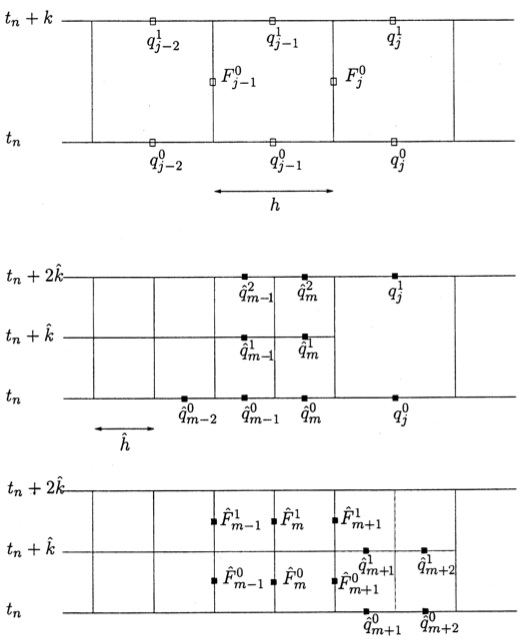
\includegraphics[width=.65\textwidth]{berg-lev-fig21}
    \caption{Essential figure for flux adapting Cartesian grids. The top grid is the normal coarse grid we are used to using with fluxes indicated. The middle diagram shows the case where a fine grid overlays a coarse grid and the interface region of fine and coarse grids. Recall that $2\hat{h}=h$ and $2\hat{k}=k$. The bottom diagram depicts the ghost cell region imposed on the coarse cell interface as well as the fine grid fluxes needed to bridge the interface.}
    \label{fig21}
\end{figure}
 
 
\subsection{Updating grid interfaces with wave propagation}
For conservation laws we have developed wave propagation methods in class whereby a Riemann problem is solved at each interface between grid cells. These methods can be extended beyond the linear accuracy to second order accuracy and controlled with limiters where smooth to discontinuous transitions occur. Wave propagation algorithms are written in a manner that they can be extended to hyperbolic problems not in conservation form retaining wave features but with no flux function. 

With flux-differencing to ensure conservation a new coarse grid value is updated by an average of fine-grid values in any cell covered by a fine grid. The key to conservation is that flux into coarse cells is accounted for by flux out of adjacent fine cells, and vice versa.
For wave-propagation algorithms, a similar correction is needed for the waves to yield conservation.  The wave-propagation form can be used to update the values at the interface between fine and coarse grid cells on each grid independently using �ghost-cell� values as needed near grid interfaces.

Whether conservative or non-conservative systems are treated, second-order corrections are still written as flux-differences and utilize the flux correction as eqn(\ref{fluxcorrect}). 
However, the first-order upwind terms written in terms of the fluctuations must be handled differently.

To maintain conservation we must {\it first} solve the Riemann problem between the ghost cell value $\hat{q}_{m+1}^{0}$ on the fine grid and the coarse grid value $q_{j}^{0}$, and add to the coarse cell value $q_{j}^{1}$ the resulting total fluctuation $A^{-}\Delta q + A^{+}\Delta q$ weighted by $\hat{k}/h = 1/2$ since the time step is $\hat{k}$ while the cell size is $h$. 
{\it Second} we must also solve a Riemann problem on the fine grid between $\hat{q}_{m+1}^{1}$ and $q_{j}^{0}$
and add these fluctuations into $q_{j}^{1}$. 

The correction step extends to an arbitrary hyperbolic system where we use a Riemann solver to obtain $A^{-}\Delta q$ and  $A^{+}\Delta q$ from the two states $\hat{q}_{m+1}^{0}$ and $q_{j}^{0}$.  This step is made in each of the $R$ time steps on the refined grid within the single coarse-grid step, where $R$ is the refinement ratio. \\

\noindent The fix-up algorithm:
\begin{description}
  \item[for $N = 0 , R-1$] \hfill \\
  solve the Riemann problem with data $\hat{q}_{m+1}^{N}$ and $q_{j}^{0}$ to compute $A^{-}\Delta q$ and  $A^{+}\Delta q$\\ \hfill
  update $q_{j}^{1} \rightarrow q_{j}^{1} + \frac{\hat{k}}{h}$ ($A^{-}\Delta q + A^{+}\Delta q$)
\end{description}


\subsection{Pseudo-code for AMR}
\subsection{Comment on determining refinement - error estimation}\label{whentorefine}
If the solution $q(x,t)$ is smooth enough, assume that our difference method $D$ has order of accuracy $s$ in both 
space and time, then the local truncation error is $q(x,t+k) -D q(x,t) = \tau(x,t) + k O(k^{s+1}+h^{s+1}))$ where $\tau$ is the leading error.
Taking two time steps suggests $q(x,t+2k) -D^2 q(x,t) = 2\tau(x,t) + k O(k^{s+1}+h^{s+1}))$.
Now, coarsen the grid to have space and time widths $2h$, $2k$ and let the differencing scheme be called $D_{2h}$ in this case. The local truncation error in this case reads $q(x,t+2k) -D_{2h} q(x,t) = 2^{s+1}\tau(x,t) + O(h^{s+2})$. Thus, an error growth estimate at time $t$ can be formed by taking the difference in the error taking two steps with the regular integration scheme, and a single large step using every other grid point:
\begin{equation}
\frac{D^2 q(x,t) - D_{2h} q(x,t)}{2^{s+1}-2} = \tau(x,t) + O(h^{s+2}) \, .
\end{equation}
The values on a grid at a given level are projected, i.e. Richardson extrapolation, onto a virtual grid coarsened by a factor of two in each direction. The solutions on both grids are advanced in time: the original grid for two time steps, the coarsened grid for one step using a time step twice as large. The difference between the solutions obtained on the two grids at each point is proportional to the local truncation error at that point. At coarse cells where the difference between the two sets of values exceed some tolerance, all four cells contained in the real grid are flagged as requiring refinement. One disadvantage of this procedure is that it always predicts a large error in the neighborhood of captured discontinuities. It is easy to construct examples for which the procedure outlined above will give values on the coarsened grid which differ pointwise by an amount independent of the mesh spacing in the neighborhood of a shock. See \cite{berg-coll} for more details. A buffer zone around the flagged cells is added to track features of interest in the refined region. This buffer zone must be affiliated with the number of time steps evaluated at a particular level. If a patch at level $L$ is refined by even integer $R_L$, then the time-step is equally refined implying that $R_L$ steps must be taken on the refined grid at level $L+1$ for each step on grid at level $L$. 

\subsection{Note on boundary conditions}

\section{Examples of 1D AMR}
\subsection{scalar advection}
The simplest problem (and most boring) is the 1D scalar advection equation
\begin{equation}
q(x,t)_{t} + \bar{u} q(x,t)_{x}=0
\end{equation}
where $\bar{u}$ is a constant representing the velocity of displacement. Let $\bar{u}>0$ for simplicity (right going).
The Riemann problem in this case consists of adding the initial conditions:
\begin{equation}
q(x,0):= \phi(x)=
\left\{ \begin{array}{c}
q_l , \, \, \, \, x<0\\
q_r , \, \, \, \, x>0\end{array}\right 
\end{equation}
\noindent Here the coefficient matrix is the number $\bar{u}$ which has eigenvalue $\lambda^1 = \bar{u}$ and eigenvector $r^1 =1$ and the jump discontinuity determined by $q_r - q_l$ propagates with speed $\lambda^1$ along characteristics. The solution is 
\begin{equation}
q(x,t):= \phi(x-\lambda^1 t) \, .
\end{equation}

\subsection{variable coefficient (color equation)}
We study here the 1D scalar problem of the form
\begin{equation}
q(x,t)_{t} + u(x) q(x,t)_{x}=0
\end{equation}
\noindent where now the velocity is allowed to vary as a function of its position. This is sometimes called the {\it color} equation.

\subsection{nonlinear scalar (Burgers)}
We study here the 1D systems derived from the conservative, 
\begin{equation}
q(x,t)_{t} + f(q(x,t))_{x}=0
\end{equation}
which can be cast in non-conservative, quasilinear form 
 \begin{equation}
q(x,t)_{t} + f'(q(x,t))q(x,t)_{x}=0 .
\end{equation}
In Burgers inviscid equation, $f(q(x,t))=\frac{1}{2}q^2$.

\subsection{linear system (acoustics)}
We study here the 1D systems of the form
\begin{equation}
q(x,t)_{t} + A q(x,t)_{x}=0
\end{equation}
\noindent and $A$ satisfies hyperbolicity conditions.

\subsection{nonlinear system (shallow water or acoustics with pressure term)}
We use the formulation in chapter 13 of \cite{levFVMHP} to describe the shallow water equations.
So, 

\begin{equation}
\left( \begin{array}{c}
h  \\
h u\end{array} \right)_{t} + 
\left( \begin{array}{c} 
hu \\
hu^2 + \frac{1}{2}gh^2\end{array} \right)_{x} = 0
\end{equation}

\noindent where $h$ is the height (or depth) of the fluid, $u$ is the horizontal component of the velocity, and $hu$ is the discharge -i.e. the flow rate of the fluid past a point. One can assign the state variables $(q^1,q^2)$, and the flux $f$ as follows: 

\begin{equation}
q(x,t)=\left( \begin{array}{c}
h  \\
h u\end{array} \right)
=
\begin{equation}
\left( \begin{array}{c}
q^1  \\
q^2\end{array} \right) 
\end{equation}
\noindent and

\begin{equation}
f(q(x,t))=
\left( \begin{array}{c} 
hu \\
hu^2 + \frac{1}{2}gh^2\end{array} \right)
= 
\left( \begin{array}{c} 
q^2 \\
(q^2)^2 / q^1 + \frac{1}{2}g (q^1)^2\end{array} \right)
\end{equation}
\noindent to be consistent with state notation from previous sections of this report.


\section{Results}
\subsection{Software implementation}
Clawpack was used to generate numerical Riemann solutions to our test problems for the fixed mesh case.
We utilized (Python, Matlab, C) for our AMR implementations.
Please find our software here: (need software + examples ...) and use the \texttt{Readme.txt} file there 
to build and test the software. The test cases presented in this report are reproduced there.
\subsection{Results of the Numerical experiments for the 1D cases}

\section{Summary}
In this paper we described the adaptive mesh refinement algorithm presented in \cite{Berger1998}, and tested the 
algorithm for several simplistic 1D cases. Our results were compared against those from Clawpack. Our AMR 
implementations are available to anyone who wants them.

%kr -just let the TOC do the outline for us and track our changes at compile time 
%also, I added a couple of bullets since our discussion this afternoon
%\section{Outline}
%\begin{itemize}
%\item Overview of paper
%\begin{itemize}
%\item Description of AMR, Figure 2.1 from Berger-Leveque paper.
%\item Wave propagation form for 1-d equations. Updating on grid interfaces, section 4 of paper
%\item pseudo-code for algorithm, similar to that on page 2310 of paper.
%\item comment on error estimation -determining refinement
%\item notes on: flagging cells, boundary conditions
%\end{itemize}
%\item Examples of 1D AMR
%\begin{itemize}
%\item scalar advection
%\item linear system (e.g. Acoustics)
%\item variable coefficient (e.g. Color equation)
%\item nonlinear scalar (burgers)
%\item nonlinear system (shallow water or acoustics with pressure term)
%\end{itemize}
%\item Results of Numerical Experiments for the 1D cases
%\item Software 
%
%\end{itemize}

\begin{thebibliography}{9}
\bibitem{claw}
http://www.clawpack.org\\

\bibitem{levFVMHP}  
  R.~Leveque
Finite Volume Methods for Hyperbolic Problems
 Cambridge University Press (2002)  \\

\bibitem{berg-coll}
M.~Berger and P.~Collela, Local Adaptive Mesh Refinement for Shock Hydrodynamics
Journal of Computational Physics 82, 64-84 (1989)\\

\bibitem{Berger1998}
M.~Berger and R.~Leveque, Adaptive Mesh Refinement Using Wave-Propagation Algorithms for Hyperbolic Systems
SIAM Journal of Numerical Analysis, 35(6):2298--2316, (1998)\\

\bibitem{Berger1982}
M.~Berger, Adaptive Mesh Refinement for Hyperbolic Partial Differential Equations,
 {\em PhD Thesis}, Department of Computer Science, Stanford University, Stanford, CA 94305 (1982)\\

\end{thebibliography}

\end{document}